\documentclass[a4paper]{article}

\usepackage{tikz}
\usetikzlibrary{positioning, arrows.meta, shapes, calc, fit, shadows}
\usepackage{float}
\usepackage{geometry}
\usepackage{xcolor}
\usepackage{amsmath}
% Use landscape and slightly narrower margins to fit the new Phase 3
\geometry{margin=0.5cm, landscape}

\begin{document}

\title{\textbf{Prescriptive Process Monitoring: Beyond Current Methods through Neuro-Symbolic Policy Distillation}}
\author{Architecture Overview}
\date{}
\maketitle

\section{System Architecture}

This diagram illustrates **Causal-Gym**, a \textbf{prescriptive process monitoring} framework that outperforms state-of-the-art methods by combining three distinct stages:
\begin{enumerate}
    \item \textbf{Initialization:} Loading AS-IS models and partial states.
    \item \textbf{Training (The Gym):} A runtime-injected simulation where an \textbf{RL Agent} explores actions, guided by \textbf{Causal Rewards} (to fix bias) and \textbf{Symbolic Guards} (to ensure safety). The agent learns a \textbf{prescriptive policy} that recommends interventions (e.g., which gateway path to take) to optimize business outcomes.
    \item \textbf{Distillation:} The complex, slow agent is "distilled" into a lightweight \textbf{Interpretable Prescriptive Policy} (Decision Tree) for sub-millisecond production inference. This final model prescribes actions in real-time.
\end{enumerate}

\begin{figure}[H]
  \centering
  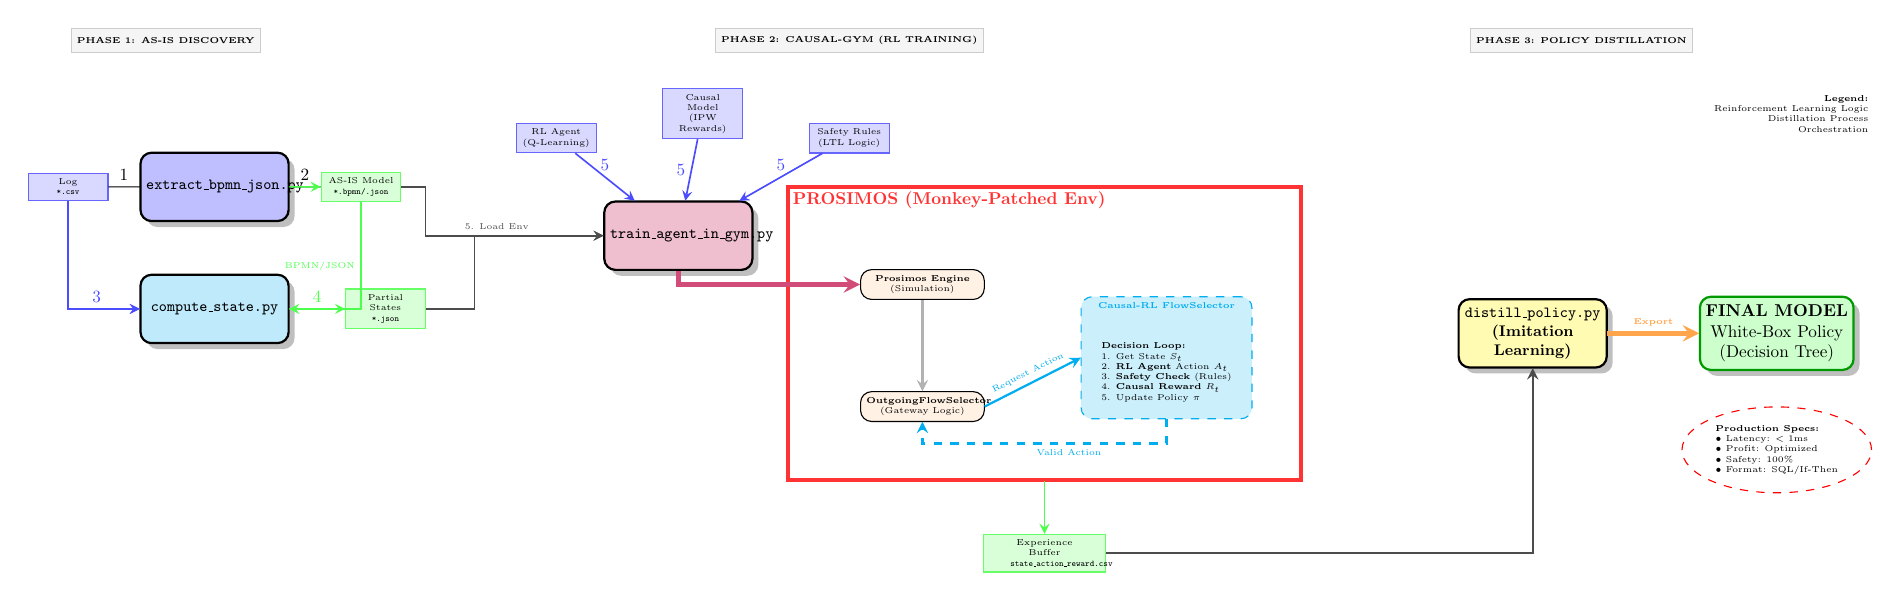
\begin{tikzpicture}[
    scale=0.62, % Slightly smaller scale to fit Phase 3
    transform shape,
    node distance=0.8cm and 1.5cm,
    script/.style={rectangle, rounded corners, draw=black, thick, 
                   minimum width=3.0cm, minimum height=1.4cm, 
                   text width=2.8cm, align=center, font=\small\bfseries, drop shadow},
    procstep/.style={rectangle, rounded corners, draw=black, fill=gray!10,
                   minimum width=2.5cm, minimum height=0.6cm,
                   text width=2.3cm, align=center, font=\tiny},
    input/.style={rectangle, draw=blue!60, fill=blue!15, 
                   minimum width=1.6cm, minimum height=0.5cm, 
                   text width=1.4cm, align=center, font=\tiny},
    output/.style={rectangle, draw=green!60, fill=green!15, 
                    minimum width=1.6cm, minimum height=0.5cm, 
                    text width=1.4cm, align=center, font=\tiny},
    tool/.style={rectangle, draw=orange!60, fill=orange!15,
                   minimum width=2cm, minimum height=0.6cm,
                   text width=1.8cm, align=center, font=\tiny},
    arrow/.style={->, >=stealth, semithick},
    phase/.style={rectangle, draw=gray!40, fill=gray!8, 
                   minimum width=3cm, minimum height=0.5cm, 
                   font=\tiny\bfseries, align=center},
    internal/.style={->, >=stealth, thin, gray!60}
  ]
    
    % Phase labels
    \node[phase] (phase1) at (-16, 10) {PHASE 1: AS-IS DISCOVERY};
    \node[phase] (phase2) at (-2, 10) {PHASE 2: CAUSAL-GYM (RL TRAINING)};
    \node[phase] (phase3) at (13, 10) {PHASE 3: POLICY DISTILLATION};
    
    % ================= PHASE 1 =================
    \node[input] (log) at (-18, 7) {Log\\\texttt{*.csv}};
    \node[script, fill=blue!25] (extract) at (-15, 7)
    {\texttt{extract\_bpmn\_json.py}};
    \draw[] (log) -- node[midway, above] {1} (extract);
    \node[script, fill=cyan!25] (compute) at (-15, 4.5) {\texttt{compute\_state.py}};
    
    \node[output] (models) at (-12, 7) {AS-IS Model\\\texttt{*.bpmn/.json}};
    \draw[] (extract) -- node[midway, above] {2} (models);
    \node[output] (states) at (-11.5, 4.5) {Partial States\\\texttt{*.json}};
    \draw[arrow, blue!70] (log) |- node[pos=0.7, above, above] {3} (compute);
    \draw[arrow, blue!70] (log) |- (compute);
    \draw[arrow, green!70] (extract) -- (models);
    \draw[arrow, green!70] (models) |- node[pos=0.3, left, font=\tiny] {BPMN/JSON} (compute);
    \draw[arrow, green!70] (compute) -- node[midway, above] {4} (states);

    % ================= PHASE 2: THE GYM =================
    
    % Orchestrator
    \node[script, fill=purple!25] (gym-script) at (-5.5, 6) {
      \texttt{train\_agent\_in\_gym.py}
    };
    
    % Inputs for RL
    \node[input] (agent) at (-8, 8) {RL Agent\\(Q-Learning)};
    \node[input] (causal) at (-5, 8.5) {Causal Model\\(IPW Rewards)};
    \node[input] (rules) at (-2, 8) {Safety Rules\\(LTL Logic)};
    
    \draw[arrow, blue!70]
      (agent) -- node[midway, above] {5} (gym-script);
    
    \draw[arrow, blue!70]
      (causal) -- node[midway, left] {5} (gym-script);
    
    \draw[arrow, blue!70]
      (rules) -- node[midway, above] {5} (gym-script);
    
    % Connecting Phase 1 to Gym
    \draw[arrow, black!70] (models.east) -- ++(0.5,0) |- node[pos=0.7, above, font=\tiny] {5. Load Env} (gym-script.west);
    \draw[arrow, black!70] (states.east) -- ++(1,0) |- (gym-script.west);

    % --- PROSIMOS ENGINE BOX ---
    \node[rectangle, draw=red!80, ultra thick, fill=white, minimum width=10.5cm, minimum height=6cm] (engine-box) at (2, 4) {};
    \node[anchor=north west, font=\bfseries, text=red!80] at (engine-box.north west) {PROSIMOS (Monkey-Patched Env)};
    
    % Engine Components
    \node[procstep, fill=orange!10] (sim-env) at (-0.5, 5) {\textbf{Prosimos Engine}\\(Simulation)};
    \node[procstep, fill=orange!10] (flow-mgr) at (-0.5, 2.5) {\textbf{OutgoingFlowSelector}\\(Gateway Logic)};
    
    % INJECTED AGENT
    \node[procstep, fill=cyan!20, dashed, draw=cyan, minimum width=3.5cm, minimum height=2.5cm] (injector) at (4.5, 3.5) {};
    \node[anchor=north, font=\tiny\bfseries, text=cyan] at (injector.north) {Causal-RL FlowSelector};
    
    % Internal Logic Text
    \node[font=\tiny, align=left, text=black] at (4.5, 3.2) {
       \textbf{Decision Loop:}\\
       1. Get State $S_t$\\
       2. \textbf{RL Agent} Action $A_t$\\
       3. \textbf{Safety Check} (Rules)\\
       4. \textbf{Causal Reward} $R_t$\\
       5. Update Policy $\pi$
    };

    % Wiring inside Engine
    \draw[internal, thick] (sim-env.south) -- (flow-mgr.north);
    \draw[internal, thick, cyan] (flow-mgr.east) -- node[above, font=\tiny, sloped, text=cyan] {Request Action} (injector.west);
    \draw[internal, thick, cyan, dashed] (injector.south) -- ++(0,-0.5) -| node[pos=0.2, below, font=\tiny, text=cyan] {Valid Action} (flow-mgr.south);
    
    % Trigger
    \draw[arrow, purple!70, ultra thick] (gym-script.south) |- (sim-env.west);

    % Gym Output
    \node[output, minimum width=2.5cm] (experience) at (2, -0.5) {Experience Buffer\\\texttt{state\_action\_reward.csv}};
    \draw[arrow, green!70] (engine-box.south) -- (experience.north);

    % ================= PHASE 3: DISTILLATION =================
    
    \node[script, fill=yellow!30] (distiller) at (12, 4) {\texttt{distill\_policy.py}\\(Imitation Learning)};
    
    \draw[arrow, black!70, thick] (experience.east) -- ++(1,0) -| (distiller.south);
    
    % Final Product
    \node[rectangle, draw=green!60!black, fill=green!20, thick, rounded corners, minimum width=3cm, minimum height=1.5cm, drop shadow, align=center] (final-model) at (17, 4) {\textbf{FINAL MODEL}\\White-Box Policy\\(Decision Tree)};
    
    \draw[arrow, orange!70, ultra thick] (distiller.east) -- node[above, font=\tiny\bfseries] {Export} (final-model.west);
    
    % Comparison Metrics Bubble
    \node[ellipse, draw=red, dashed, fill=white, align=left, font=\tiny, anchor=north] at (17, 2.5) {
        \textbf{Production Specs:}\\
        $\bullet$ Latency: $<1$ms\\
        $\bullet$ Profit: Optimized\\
        $\bullet$ Safety: 100\%\\
        $\bullet$ Format: SQL/If-Then
    };

    % LEGEND
    \node[anchor=north east, font=\tiny, align=right] at (19, 9) {
        \textbf{Legend:}\\
        \textcolor{cyan!80}{$\blacksquare$} Reinforcement Learning Logic\\
        \textcolor{yellow!80}{$\blacksquare$} Distillation Process\\
        \textcolor{purple!80}{$\blacksquare$} Orchestration
    };

  \end{tikzpicture}
  \caption{The \textbf{Causal-Gym Architecture} (Prescriptive Process Monitoring). Unlike standard approaches that deploy heavy black-box models, this system uses a three-stage pipeline. (1) We prepare the environment. (2) We inject a \textbf{Causal-RL Agent} into the simulation runtime; this agent explores the solution space, optimizing for Net Gain using IPW-adjusted rewards while constrained by Symbolic Safety Rules. The agent learns a \textbf{prescriptive policy} that recommends interventions (actions) at runtime. (3) The resulting high-performance (but slow) agent generates a massive experience buffer, which is \textbf{distilled} into a lightweight, interpretable Decision Tree. This final \textbf{prescriptive model} beats the SOTA in profit (via RL) while matching the speed of simple heuristics (via Distillation).}
  \label{fig:causal-gym}
\end{figure}

\newpage

\section{Technical Defense: How Causal-Gym Beats the Benchmark}

This architecture is specifically engineered to address the trade-offs present in current literature (SOTA), providing a "Best of All Worlds" solution.

\subsection{Phase 2: The Causal-RL Gym (Maximizing Profit)}
Most approaches are either "Induced" (myopic) or "Learned" (blind to causality).
\begin{itemize}
    \item \textbf{Monkey-Patching as an Environment:} We transform the \texttt{Prosimos} simulator into an OpenAI Gym-compatible environment. By replacing the \texttt{OutgoingFlowSelector} at runtime, the RL agent can interact with the process dynamics directly.
    \item \textbf{Causal Rewards (IPW):} Standard RL overfits to historical data biases. We integrate a Causal Estimator (Inverse Propensity Weighting) into the reward function. 
    \[ R_t = \text{Revenue} - \text{Cost} + \text{CausalCorrection}(A_t, X_t) \]
    This ensures the agent learns the \textit{true} effect of interventions, surpassing methods like \textit{Learning When to Treat} in robustness.
    \item \textbf{Symbolic Safety Layer \& Constraints:} An LTL (Linear Temporal Logic) monitor intercepts every action. It enforces not only logical compliance but also \textbf{resource constraints} (e.g., "Max 5 interventions per hour"). If an action violates a rule or budget, it is masked out. This solves the optimization problem under constraints better than Knapsack approaches, as the agent learns to preserve budget for high-value cases.
\end{itemize}

\subsection{Phase 3: Policy Distillation (Minimizing Latency)}
A major criticism of RL in BPM is inference latency (often $>100$ms).
\begin{itemize}
    \item \textbf{The Bottleneck:} Running a Simulation + Neural Network + LTL Monitor for every single transaction is too slow for real-time payment processing.
    \item \textbf{The Solution (Distillation):} We treat the Phase 2 Agent as a "Teacher". We generate millions of optimal decisions in the simulator (offline). Then, we train a "Student" model—a simple \textbf{Decision Tree} or \textbf{Rule List}—to mimic the Teacher.
    \item \textbf{The Result:} The final artifact is a static set of \texttt{IF-THEN} rules.
    \begin{itemize}
        \item \textbf{Latency:} $<1$ms (CPU). Beats \textit{Intervening with Confidence}.
        \item \textbf{Explainability:} Native. Beats Black-box Deep Learning.
        \item \textbf{Deployment:} Can be implemented in SQL or Java without Python dependencies.
    \end{itemize}
\end{itemize}

\end{document}